\documentclass[11pt,a4paper]{article}

% ---------------------------------------------------------------------------
% Packages
% ---------------------------------------------------------------------------
\usepackage[margin=2.5cm]{geometry}
\usepackage[utf8]{inputenc}
\usepackage[T1]{fontenc}
\usepackage{graphicx}
\usepackage{tikz}
\usetikzlibrary{shapes.geometric, arrows.meta, positioning, fit, backgrounds, calc}
\usepackage{booktabs}
\usepackage{xcolor}
\usepackage{hyperref}
\usepackage{listings}
\usepackage{enumitem}
\usepackage{caption}
\usepackage{float}
\usepackage{parskip}
\usepackage{underscore}
\usepackage[export]{adjustbox}

\hypersetup{
    colorlinks=true,
    linkcolor=blue!50!black,
    citecolor=blue!50!black,
    urlcolor=blue!50!black,
    pdftitle={Phase 2 Implementation Report -- Recommender API Contract and Query Log},
    pdfauthor={Narges}
}

% ---------------------------------------------------------------------------
% Color palette for diagrams (same palette as the Phase 0/1 and Phase 3 reports)
% ---------------------------------------------------------------------------
\definecolor{dbcolor}{RGB}{215,235,250}
\definecolor{apicolor}{RGB}{255,235,205}
\definecolor{harnesscolor}{RGB}{225,245,225}
\definecolor{pipelinecolor}{RGB}{240,225,245}
\definecolor{outcolor}{RGB}{255,225,225}
\definecolor{boxborder}{RGB}{80,80,80}

\tikzset{
    block/.style={rectangle, draw=boxborder, rounded corners, thick,
        text width=3.2cm, minimum height=1.1cm, align=center, font=\small},
    smallblock/.style={rectangle, draw=boxborder, rounded corners, thick,
        text width=2.6cm, minimum height=0.9cm, align=center, font=\footnotesize},
    arrow/.style={-{Latex[length=2.5mm]}, thick}
}

% ---------------------------------------------------------------------------
% Listings style
% ---------------------------------------------------------------------------
\lstset{
    basicstyle=\ttfamily\footnotesize,
    breaklines=true,
    frame=single,
    backgroundcolor=\color{gray!7},
    columns=fullflexible,
    showstringspaces=false,
    xleftmargin=1em,
    xrightmargin=1em,
    aboveskip=8pt,
    belowskip=8pt
}

\newcommand{\code}[1]{\texttt{#1}}

\title{\Large \textbf{A Query Recommender for Preference-Aware Natural Language Querying} \\[4pt]
\large Implementation Report --- Phase 2 (Recommender API Contract \& Query Log Store) \\[2pt]
\normalsize \emph{The persistence and contract layer the recommender core is built inside}}
\author{Narges \\ \small Supervisor: Prof. Elisa Quintarelli}
\date{\today}

\begin{document}

\maketitle

\begin{abstract}
\noindent
This report documents Phase 2 of the thesis: a fixed \textbf{request/response contract} for the
query recommender, exposed as \code{POST /recommend}, and a \textbf{persistent, user-keyed query
log} that every call to it appends to. Per the scope decision recorded in the companion
\emph{Phase 0 \& Phase 1 Implementation Report}, the thesis's entire contribution is the
recommender delivered as a standalone model and API --- Phase 2 is the boundary that makes this
possible: it fixes the interface external callers integrate against and builds the persistence
layer the recommender core (Phase 4) is built inside, before any recommendation logic exists
behind it. This report explains what was built, a deliberate deviation from the roadmap's literal
wording concerning how the internal development harness exercises the contract, and the
verification performed on both the real HTTP path and the in-process path the harness uses.
\end{abstract}

\tableofcontents
\newpage

% =============================================================================
\section{Introduction}
% =============================================================================

Following the scope narrowing agreed with the supervisor (documented in full in the \emph{Phase 0
\& Phase 1 Implementation Report}), the thesis's deliverable is not a user interface but a
\textbf{standalone recommender API}: any calling application --- the bachelor students' domain/
user-selection app, or this repository's own development harness --- integrates the recommender
by calling an endpoint. Before any recommendation logic can be built, that endpoint's
\textbf{contract} must be fixed and a place to \textbf{persist queries} must exist, since the
recommender's core technique (Section~\ref{sec:where}) depends on retrieving a user's own past
queries. Phase 2 delivers exactly these two things, and nothing else: candidate generation itself
is Phase 4.

\subsection{Scope}

Phase 2 is domain-agnostic by design: the contract and the log store accept any \code{domain}
string and encode no Movie- or Tourism-specific assumptions. This mirrors the roadmap's own
framing of the recommender as a single model serving both domains, rather than two
domain-specific implementations.

\subsection{Where this fits}
\label{sec:where}

Phase 2 is implemented in a new \code{recommender/api/} package, alongside the already-existing
\code{recommender/behavioral\_profile.py} (Phase 3) as a sibling module in the same top-level
\code{recommender/} package --- the standalone deliverable per the scope decision. Its output, a
persistent per-user query log, is the direct input to Phase 4a's retrieval-augmented candidate
generation (RA-GQR style): the recommender retrieves a user's own semantically similar past
queries from this log to build its generation prompt, described in the project roadmap and in the
companion \emph{Phase 4 Implementation Report}.

\newpage
% =============================================================================
\section{High-Level Overview}
% =============================================================================

\subsection{The core idea}

Phase 2 stands up a stable boundary --- one request shape in, one response shape out --- before
any of the logic behind it exists, so that:

\begin{enumerate}[label=(\alph*)]
    \item external callers can integrate against a fixed contract independently of when Phase 4's
        recommendation logic lands;
    \item every answered query is durably logged, keyed by user and domain, so later phases have
        real per-user history to retrieve from instead of starting cold; and
    \item the internal development harness (\code{gui\_v2.py}) can exercise the same contract a
        real external caller would use, without requiring a second always-running server process
        during local development (Section~\ref{sec:design}).
\end{enumerate}

\subsection{Pipeline diagram}

Figure~\ref{fig:overview} shows how a request reaches the shared handler function and where it is
persisted. Both callers --- the real HTTP endpoint and the in-process development harness ---
converge on the same function, \code{handle\_recommend()}, which is the single extension point
later phases build inside.

\begin{figure}[H]
\centering
\begin{adjustbox}{max width=\textwidth, max totalheight=0.85\textheight, center}
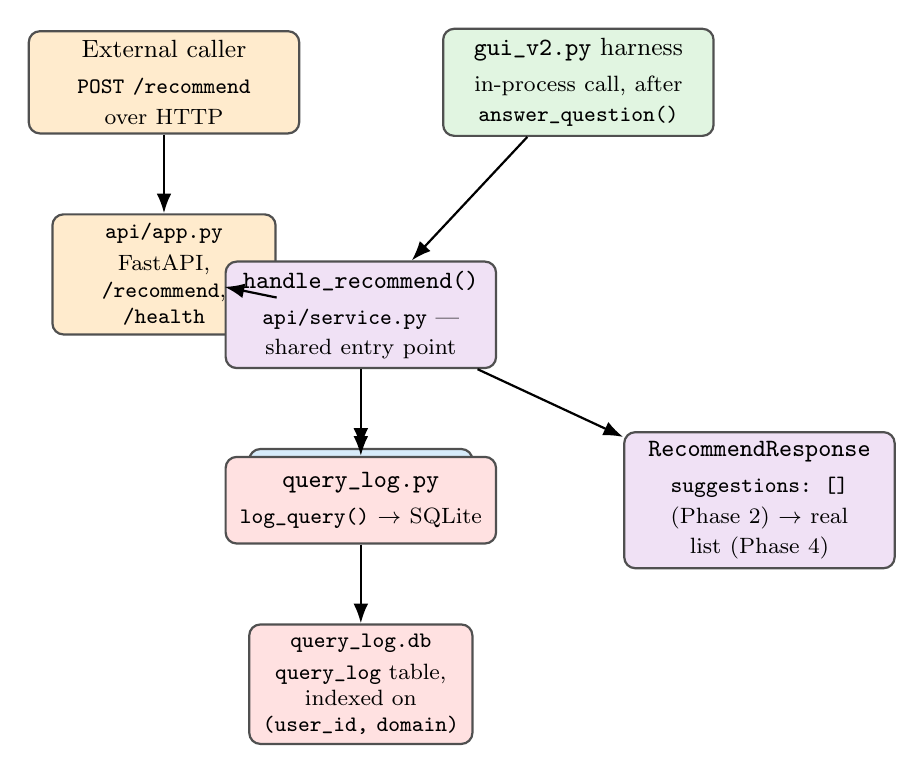
\begin{tikzpicture}[node distance=1.0cm and 1.4cm]

    \node[block, fill=apicolor] (http) {External caller\\[2pt]\footnotesize \code{POST /recommend} over HTTP};
    \node[block, fill=harnesscolor, right=1.8cm of http] (gui) {\code{gui\_v2.py} harness\\[2pt]\footnotesize in-process call, after \code{answer\_question()}};

    \node[smallblock, fill=apicolor, below=of http] (app) {\code{api/app.py}\\[2pt]\footnotesize FastAPI, \code{/recommend}, \code{/health}};

    \node[block, fill=pipelinecolor, below=1.6cm of http, xshift=2.5cm] (handle) {\code{handle\_recommend()}\\[2pt]\footnotesize \code{api/service.py} --- shared entry point};

    \node[smallblock, fill=dbcolor, below=of handle] (schemas) {\code{RecommendRequest}\\[2pt]\footnotesize pydantic validation};

    \node[block, fill=outcolor, below=1.1cm of handle] (log) {\code{query\_log.py}\\[2pt]\footnotesize \code{log\_query()} $\to$ SQLite};

    \node[smallblock, fill=outcolor, below=of log] (db) {\code{query\_log.db}\\[2pt]\footnotesize \code{query\_log} table, indexed on \code{(user\_id, domain)}};

    \node[block, fill=pipelinecolor, right=1.6cm of log] (resp) {\code{RecommendResponse}\\[2pt]\footnotesize \code{suggestions: []} (Phase 2) $\to$ real list (Phase 4)};

    \draw[arrow] (http) -- (app);
    \draw[arrow] (app) -- (handle);
    \draw[arrow] (gui) -- (handle);
    \draw[arrow] (handle) -- (schemas);
    \draw[arrow] (handle) -- (log);
    \draw[arrow] (log) -- (db);
    \draw[arrow] (handle) -- (resp);

\end{tikzpicture}
\end{adjustbox}
\caption{Phase 2 data flow. Both the real HTTP endpoint and the in-process development harness
converge on \code{handle\_recommend()}, which validates the request, persists it to the SQLite
query log, and returns a response --- an empty suggestion list in this phase, since candidate
generation is Phase 4.}
\label{fig:overview}
\end{figure}

\newpage
% =============================================================================
\section{Detailed Walkthrough}
% =============================================================================

\subsection{The contract (\code{recommender/api/schemas.py})}

\begin{lstlisting}[language=Python, caption={The recommender's request/response contract, matching
the roadmap's Phase 2 sketch exactly, with one field left deliberately open.}]
class RecommendRequest(BaseModel):
    user_id: str
    domain: str
    query_text: str
    generated_sparql: Optional[str] = None
    result_summary: Optional[Any] = None
    interaction_data: Optional[dict] = None

class RecommendResponse(BaseModel):
    suggestions: list[str] = Field(default_factory=list)
\end{lstlisting}

One field is a deliberate, documented gap: \code{interaction\_data} stays an untyped
\code{Optional[dict]} rather than a fixed schema, because its real shape depends on an open
dependency --- what the bachelor students' external application actually logs per user (queries,
clicks, dwell time, and so on). That confirmation has not happened, so typing it further now would
mean guessing at a contract that might not match reality; Phase 3's \code{netflix\_dataset}-derived
behavioral profiles are the practical stand-in signal used instead (Section~\ref{sec:limits}).

\subsection{The query log store (\code{recommender/query\_log.py})}

A single SQLite table, created on first use:

\begin{lstlisting}[language=SQL, caption={The query log schema. SQLite was chosen deliberately
over Postgres: a single-file, zero-infrastructure store is appropriate for a thesis-scale log that
does not need to be shared across processes beyond one local API server, consistent with the
project's existing pattern of using the lightest tool that fits (e.g.\ JSON-per-user files in
Phase 3, not a database).}]
CREATE TABLE query_log (
    id INTEGER PRIMARY KEY AUTOINCREMENT,
    user_id TEXT NOT NULL,
    domain TEXT NOT NULL,
    query_text TEXT NOT NULL,
    timestamp TEXT NOT NULL,
    generated_sparql TEXT,
    result_summary TEXT
);
CREATE INDEX idx_query_log_user_domain ON query_log(user_id, domain);
\end{lstlisting}

Two functions cover the read and write side:

\begin{itemize}
    \item \code{log\_query(user\_id, domain, query\_text, generated\_sparql=None,
        result\_summary=None, timestamp=None)} --- appends one row. \code{timestamp} defaults to
        UTC now if not supplied; \code{result\_summary} is JSON-serialized automatically when
        given a dict or list, so callers can pass structured summaries (e.g.\
        \code{\{"row\_count": 12\}}) without pre-serializing them.
    \item \code{get\_user\_history(user\_id, domain=None, limit=50)} --- the most recent rows for
        a user, optionally scoped to one domain. This is the function Phase 4a's
        embedding-based similar-query retrieval calls to build its candidate pool.
\end{itemize}

\subsection{The request handler (\code{recommender/api/service.py})}

\begin{lstlisting}[language=Python, caption={\code{handle\_recommend()} as implemented in Phase 2
--- validate and persist only. Phase 4 replaces the final line with the real retrieval $\to$ LLM
generation $\to$ schema-validation $\to$ ranking pipeline, without changing this function's
signature.}]
def handle_recommend(request: RecommendRequest) -> RecommendResponse:
    log_query(
        user_id=request.user_id,
        domain=request.domain,
        query_text=request.query_text,
        generated_sparql=request.generated_sparql,
        result_summary=request.result_summary,
    )
    return RecommendResponse(suggestions=[])
\end{lstlisting}

This function is the single place both the HTTP endpoint and the development harness call
(Section~\ref{sec:design}). Its only job in this phase is to validate the request shape (via
pydantic) and persist it; \code{suggestions} is always \code{[]} here, by design --- the contract,
log store, and harness wiring exist specifically so Phase 4 can be implemented purely inside this
one function.

\subsection{The FastAPI application (\code{recommender/api/app.py})}

\begin{lstlisting}[language=Python, caption={The HTTP surface: a thin FastAPI wrapper around
\code{handle\_recommend()}. Run with \code{uvicorn recommender.api.app:app --reload --port 8000}
from the repo root.}]
app = FastAPI(title="Query Recommender API", version="0.1.0")

@app.get("/health")
def health(): ...

@app.post("/recommend", response_model=RecommendResponse)
def recommend(request: RecommendRequest) -> RecommendResponse:
    return handle_recommend(request)
\end{lstlisting}

OpenAPI documentation is auto-served at \code{/docs}, generated for free by FastAPI from the
pydantic models above --- satisfying, early and at no extra cost, the roadmap's later note that
the API should be documented well enough that external integration does not require reading the
source.

\subsection{Harness integration (\code{web\_app/nl2sparql/gui\_v2.py})}

Three changes were made to the development harness, all additive:

\begin{enumerate}
    \item \textbf{Import path}. \code{recommender/} lives at the repository root, a sibling of
        \code{web\_app/}, not a subpackage of it. \code{gui\_v2.py} inserts
        \code{Path(\_\_file\_\_).resolve().parents[2]} (the repository root) onto \code{sys.path}
        before importing \code{recommender.api.schemas}/\code{recommender.api.service}, guarded by
        a \code{try/except ImportError} so the rest of the harness still works if the
        \code{recommender} package is not importable for some reason.
    \item \textbf{User picker}. A new ``User'' sidebar section, placed directly after domain
        selection, with a text input bound to \code{st.session\_state.user\_id}, defaulting to
        \code{"user\_00001"} --- chosen to match the Movie-domain behavioral-profile id scheme, so
        a developer can immediately cross-reference a Phase 3 profile with the id typed here.
    \item \textbf{Post-query call}. After \code{process\_question()} returns and results are
        displayed, the harness builds a \code{RecommendRequest} from the just-answered question
        (\code{user\_id} from the sidebar, \code{domain} from the active domain,
        \code{generated\_sparql} and a \code{\{"row\_count": ...\}} summary from the pipeline's
        own results) and calls \code{handle\_recommend()}, rendering a new ``Suggested Follow-up
        Queries'' section. Since \code{suggestions} is always empty in this phase, the section
        currently shows a caption noting the query was logged for a not-yet-implemented
        recommender, rather than a suggestion list. The call is wrapped in a \code{try/except} so
        a recommender-side failure never breaks the pipeline-results display the rest of the
        harness depends on.
\end{enumerate}

\newpage
% =============================================================================
\section{Design Decision: In-Process Call, Not HTTP, From the Harness}
\label{sec:design}
% =============================================================================

The roadmap's Phase 2 bullet, read literally, could be taken to mean the development harness
should make a real HTTP \code{POST http://localhost:8000/recommend} call to a separately-running
\code{uvicorn} process, to ``exercise the same API contract end-to-end during development.'' That
was deliberately not what was implemented. Instead, \code{handle\_recommend()} is a plain Python
function, imported directly by both \code{recommender/api/app.py} (for the real HTTP endpoint) and
\code{gui\_v2.py} (for the harness). The reasoning:

\begin{itemize}
    \item \textbf{The contract is identical either way.} The request/response \emph{shape} ---
        the actual thing ``exercising the contract'' is meant to validate --- is the same whether
        it is invoked over HTTP or as a direct function call, since both paths go through the same
        pydantic models and the same \code{handle\_recommend()} logic.
    \item \textbf{Less development friction.} Requiring a Streamlit developer to also keep a
        second \code{uvicorn} process running, healthy, and pointed at the same
        \code{query\_log.db}, just to see a suggestions section render during
        \code{streamlit run}, is friction the contract does not need to impose.
        \code{NL2SPARQLPipeline.answer\_question()} itself was also left unmodified --- the
        recommender call happens in \code{gui\_v2.py} \emph{after} \code{answer\_question()}
        returns, because it needs the finished SPARQL query and result count as inputs, which do
        not exist until the pipeline has already run.
    \item \textbf{The real HTTP path was still built and verified independently}
        (Section~\ref{sec:verification}) --- external callers such as the bachelor students'
        application are unaffected by this choice; they only ever see the HTTP surface.
\end{itemize}

If a future need arises to test the actual HTTP transport realistically (e.g.\ once a later phase
adds latency or timeout behavior worth exercising), swapping the harness's direct call for a
\code{requests.post(...)} call is a small, isolated change --- the contract itself does not move.

\newpage
% =============================================================================
\section{Verification Performed}
\label{sec:verification}
% =============================================================================

\subsection{HTTP path}

\code{uvicorn recommender.api.app:app --port 8000} was started from the repository root.

\begin{lstlisting}[language=, caption={HTTP verification of both endpoints.}]
POST /recommend  {"user_id":"user_00001","domain":"movie","query_text":"Action movies",
                   "result_summary":{"count":3}}
-> 200 {"suggestions":[]}

GET /health
-> 200 {"status":"ok"}
\end{lstlisting}

The corresponding row was confirmed present in \code{recommender/output/query\_log.db}:

\begin{lstlisting}[language=, caption={The persisted row for the request above.}]
{'id': 1, 'user_id': 'user_00001', 'domain': 'movie', 'query_text': 'Action movies',
 'timestamp': '2026-07-25T15:19:10.007544+00:00', 'generated_sparql': None,
 'result_summary': '{"count": 3}'}
\end{lstlisting}

\subsection{In-process path}

Mirroring exactly how \code{gui\_v2.py} imports the package, a second request was issued from a
working directory of \code{web\_app/} (matching where Streamlit actually runs from), inserting the
repository root onto \code{sys.path} the same way \code{gui\_v2.py}'s
\code{Path(\_\_file\_\_).resolve().parents[2]} does, then importing
\code{recommender.api.service.handle\_recommend} and calling it directly. A second row
(\code{id=2}, \code{user\_id="user\_00002"}) was confirmed appended to the same
\code{query\_log.db} --- proving the import resolution the harness relies on actually works from
its real runtime working directory, not merely from the repository root.

\subsection{Static check}

\code{ast.parse()} on the full, edited \code{gui\_v2.py} succeeded after the harness changes,
confirming no syntax errors were introduced by the new sidebar section or the post-query call
block.

\subsection{Not done in this pass}

A full manual Streamlit click-through of the new sidebar field and suggestions section was not
performed (no browser automation tool was available in this environment --- the same limitation
noted in the Phase 0/1 verification record). Worth a quick manual sanity pass before relying on
this for a live demo.

% =============================================================================
\section{Interpretation and Limitations}
\label{sec:limits}
% =============================================================================

\begin{itemize}
    \item \textbf{\code{suggestions} is always \code{[]}.} This is expected and correct for this
        phase --- Phase 4 is where candidate generation happens. The contract, log store, and
        harness wiring are all in place specifically so Phase 4 can be implemented purely inside
        \code{handle\_recommend()} without touching the API surface or the harness again, which is
        exactly what happened (see the companion \emph{Phase 4 Implementation Report}).
    \item \textbf{\code{interaction\_data} is unused so far.} Neither \code{handle\_recommend()}
        nor the harness populates or reads it yet; it exists in the contract as a placeholder for
        the still-unconfirmed shape of what the external application logs. Until that is
        confirmed, Phase 3's \code{netflix\_dataset}-derived behavioral profiles (keyed by the
        same \code{user\_id} convention used in the harness's default) are the practical stand-in
        signal Phase 4 conditions on instead.
    \item \textbf{SQLite is a single-writer store.} Appropriate for one local development API
        process; if this ever needed to serve concurrent write-heavy traffic (unlikely at
        thesis-demo scale), it would need revisiting --- not a requirement raised by the
        supervisor or anywhere in the roadmap, noted here only for completeness.
    \item \textbf{No authentication, rate-limiting, or input sanitization beyond pydantic's type
        validation} --- appropriate for a thesis-scope local development API, not a production
        deployment, and not called out as a requirement anywhere in the roadmap.
\end{itemize}

% =============================================================================
\section{Summary and Next Steps}
% =============================================================================

Phase 2 delivers a fixed, verified contract (\code{POST /recommend}, \code{GET /health}) and a
persistent, user-keyed query log, exercised successfully both over real HTTP and through the
in-process path the development harness uses --- with the deliberate design choice
(Section~\ref{sec:design}) that both paths share one function, \code{handle\_recommend()}, so later
phases only need to change one place.

\textbf{Phase 4} (documented separately in the \emph{Phase 4 Implementation Report}) is the direct
consumer of this phase's output: query-log retrieval (\code{get\_user\_history()}), candidate
generation, schema-grounding validation, and ranking are all implemented inside
\code{handle\_recommend()}, replacing its final line without any change to the contract, the log
store, or the harness wiring built here. Full detail on Phase 3 (the behavioral signal Phase 4 also
conditions on) and Phase 4 onward is tracked in the project roadmap document, \emph{Thesis Project
Plan}.

\end{document}
